\documentclass{article}
\usepackage[utf8]{inputenc}
\usepackage{amsmath}
\usepackage{amssymb}
\usepackage{graphicx}

\begin{document}

\section*{Adaptive Interpolation of Closed Curves}
A $1$-periodic continuously differentiable function  $\mathbf{c}: \mathbb{R} \to \mathbb{R}^{2}$ parameterizes a closed curve in the plane.

\begin{figure}[!hbt]
    \centering
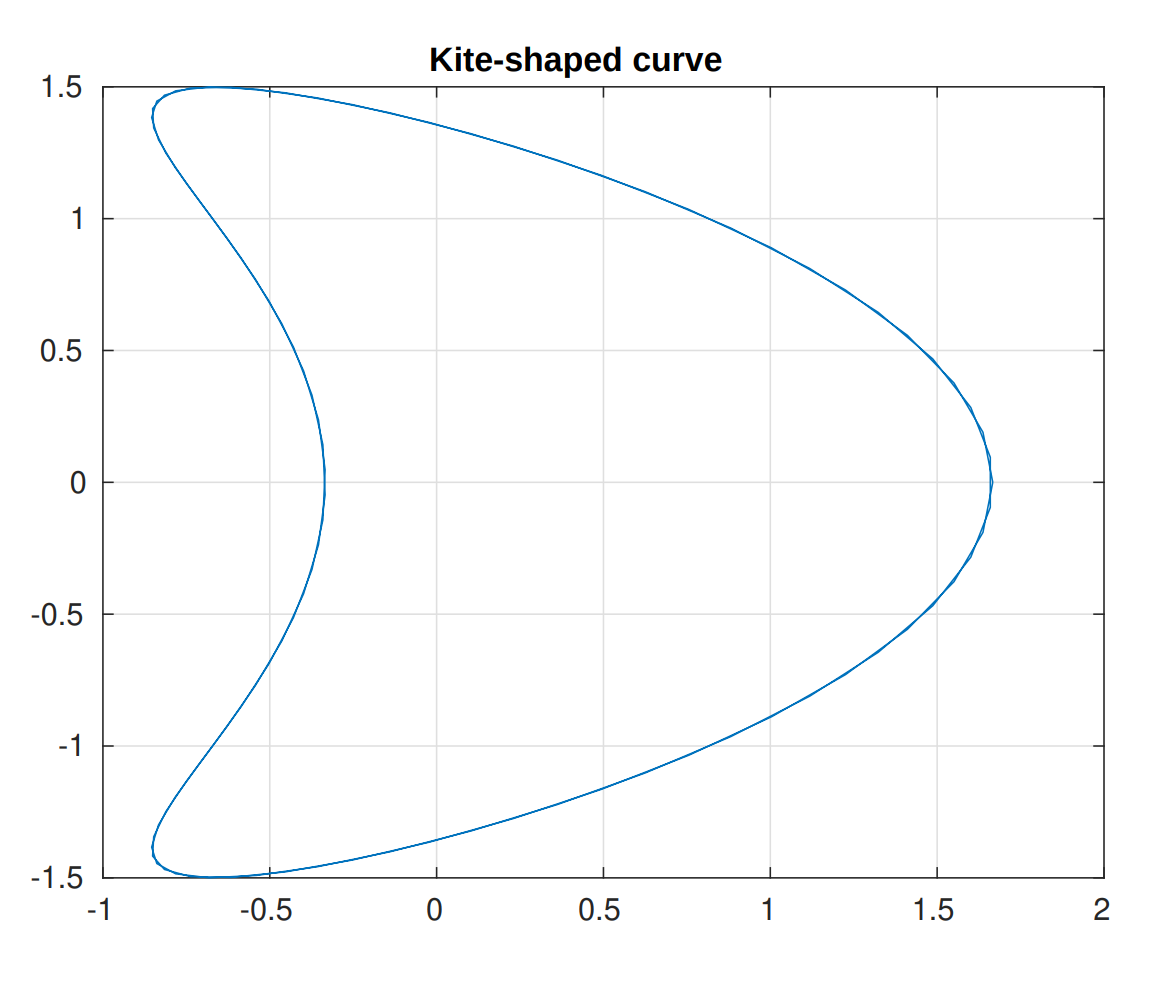
\includegraphics[width=0.4\linewidth]{KiteShapedCurve.png}
\end{figure}

The above kite-shaped curve is paramterized by 
\begin{equation*}
    \mathbf{c}\left(t\right) = \begin{bmatrix}
    \cos\left(2\pi t\right) + \frac{2}{3}\cos\left(4\pi t\right) \\
    \frac{3}{2} \sin\left(2\pi t\right)
    \end{bmatrix}
\end{equation*}

We denote for a polygon shape defined by a given sequence of $n \geq 2$ mutually distinct points $\left(\mathbf{p}_{1}, \mathbf{p}_{2}, \dots, \mathbf{p}_{n}\right)$ in the plane with $\mathbf{p}_{k} \in \mathbb{R}^{2}$
\begin{align*}
    \delta_{i} &:= \left\lVert \mathbf{p}_{i+1} - \mathbf{p}_{i} \right\rVert \, ,\quad i = 1, \dots, n-1 \qquad
    &&\delta_{n} := \left\lVert \mathbf{p}_{1} - \mathbf{p}_{n} \right\rVert \\
    \lambda_{0} &:= 0 \qquad
    &&\lambda_{k} := \sum_{j=1}^{k} \delta_{j}\,,\quad k = 1,\dots, n \\
    \mathbf{d}_{i} &:= \mathbf{p}_{i+1} - \mathbf{p}_{i}\,,\quad i=1, \dots, n-1 \qquad
    &&\mathbf{d}_{n} := \mathbf{p}_{1} - \mathbf{p}_{n} \\
    \mathbf{t}_{i} &:= \frac{\mathbf{d}_{i}}{\left\lVert \mathbf{d}_{i}\right\rVert}\,,\quad i = 1, \dots, n
\end{align*}

\begin{figure}[!hbt]
    \centering
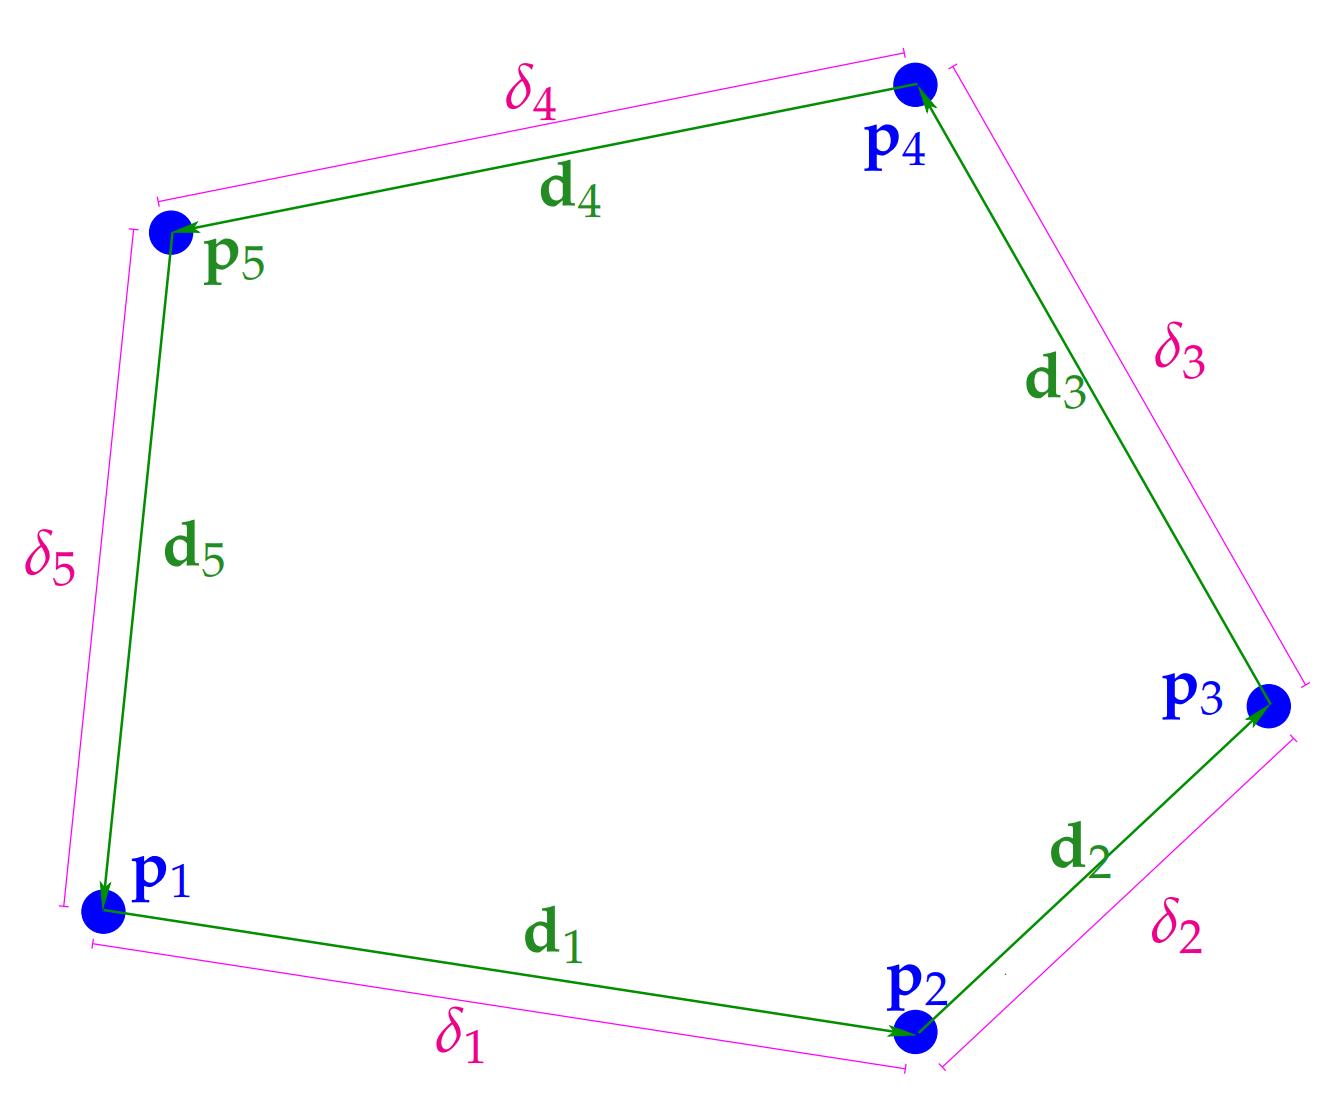
\includegraphics[width=0.5\linewidth]{PointConnectedCurve.png}
\end{figure}

We study two ways to connect points in the plane by a piecewise polynomial closed curve

\pagebreak

\noindent The first one is given by

\begin{figure}[!hbt]
    \centering
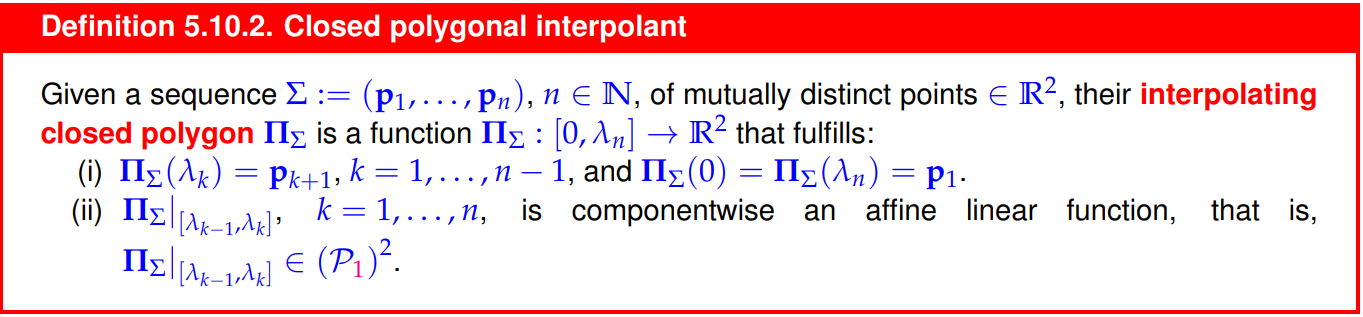
\includegraphics[width=1.0\linewidth]{ClosedPolynomialInterpolant.png}
\end{figure}

\noindent And the second one is given by

\begin{figure}[!hbt]
    \centering
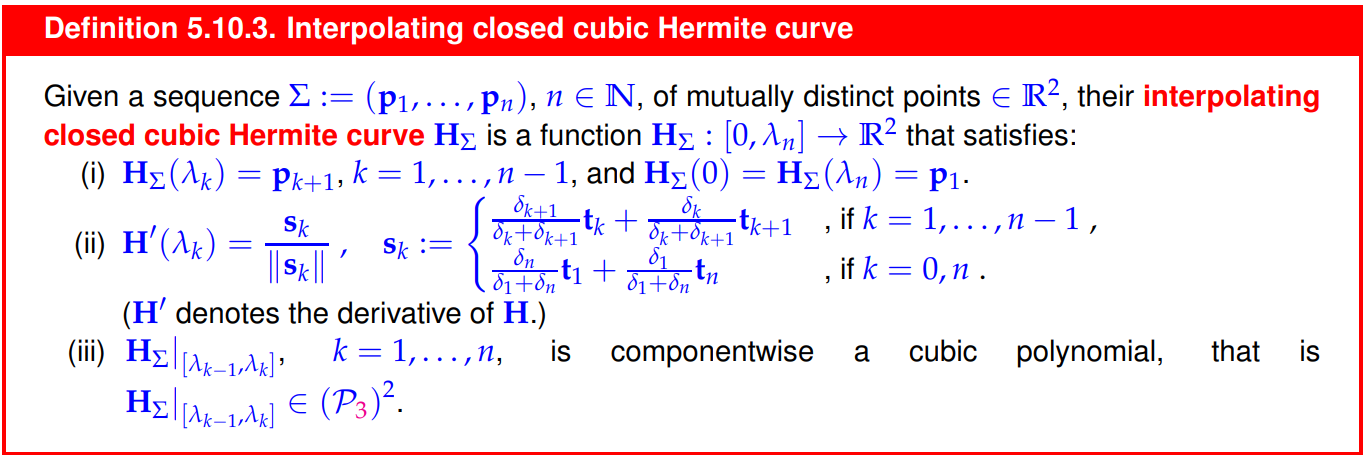
\includegraphics[width=1.0\linewidth]{InterpolatingClosedCubicHermiteCurve.png}
\end{figure}

\subsection*{5-10.a}
We are tasked with writing a function that takes a vector of points \verb|Sigma| and a vector of sorted values $x_{i}$ and returns their interpolating closed polygon. We have $\Sigma := \left(\mathbf{p}_{1}, \dots, \mathbf{p}_{n}\right)$ and $\mathbf{x} = \left(x_{1}, \dots, x_{n}\right)$. We are tasked with returning a sequence of coordinates $\mathbf{\Pi}_{\Sigma}\left(x_{k} \lambda_{n}\right)$ for $k = 1, \dots, M$, where $M$ is the length of the vector $\mathbf{x}$. We first use the notations defined above to compute the values needed. We do the following (we will set $\Sigma_{n} = \Sigma_{0}$ in the code which will make it easier to work with the given formulae.)
\begin{enumerate}
    \item First compute $\mathbf{d}_{i} = \mathbf{p}_{i+1} - \mathbf{p}_{i}$.
    \item Use $\mathbf{d}_{i}$ computed before to compute $\delta_{i} = \left\lVert \mathbf{p}_{i+1} - \mathbf{p}_{i} \right\rVert = \left\lVert \mathbf{d}_{i}
    \right\rVert$
    \item We have $\delta_{0} = 0$ and $\delta_{k} = \sum_{j=1}^{k}\delta_{j}$ for $k = 1, \dots, n$, we hence compute at the step $i > 0$ the next lambda value as $\lambda_{i} = \lambda_{i-1} + \delta_{i}$
\end{enumerate}
We then now that the points are connected by straight lines, hence we can use the piecewise linear interpolant formula to interpolate the values $x_{1}, \dots, x_{M}$ onto the curve given by $\Pi_{\Sigma}$. We for this need to match the points given in $\mathbf{x}$ to the corresponding correct two points on the polygon. For this we iterate over all points on the polygon and check if any of the points (scaled by a factor of $\lambda_{n}$) in $\mathbf{x}$ lie between two points, if that is the case we can then apply piecewise linear interpolation. 

\pagebreak 

\noindent The formula for piecewise linear interpolation is given in the lecture document as
\begin{equation*}
    s\left(t\right) = \frac{\left(t_{i+1}-t\right)y_{i} + \left(t-t_{i}\right)y_{i+1}}{t_{i+1} - t_{i}} \quad \text{for} \quad t\in \left[t_{i}, t_{i+1}\right]
\end{equation*}
we can see that here we have $x_{j}\lambda_{n} = t$ in each iteration. We will want to find $i$ such that 
\begin{equation*}
    \lambda_{i-1} \leq x_{j}\lambda_{n} \leq \lambda_{i}
\end{equation*}
this will then translate to the resulting point being between $\mathbf{p}_{i-1}$ and $\mathbf{p}_{i}$. We hence get the formula
\begin{equation*}
    \mathbf{s}\left(x_{j}\right) = \frac{\left(\lambda_{i} - x_{j}\lambda_{n}\right)\Sigma_{i-1}+ \left(x_{j}\lambda_{n} - \lambda_{i-1}\right)\Sigma_{i}}{\left\lVert \mathbf{p}_{i} - \mathbf{p}_{i-1}\right\rVert} = \frac{\left(\lambda_{i} - x_{j}\lambda_{n}\right)\Sigma_{i-1}+ \left(x_{j}\lambda_{n} - \lambda_{i-1}\right)\Sigma_{i}}{\delta_{i-1}}
\end{equation*}
For whatever reason they tend to love not to use this formula in the solutions, I believe that this is equivalent. This produces the following code.
\begin{figure}[!hbt]
    \centering
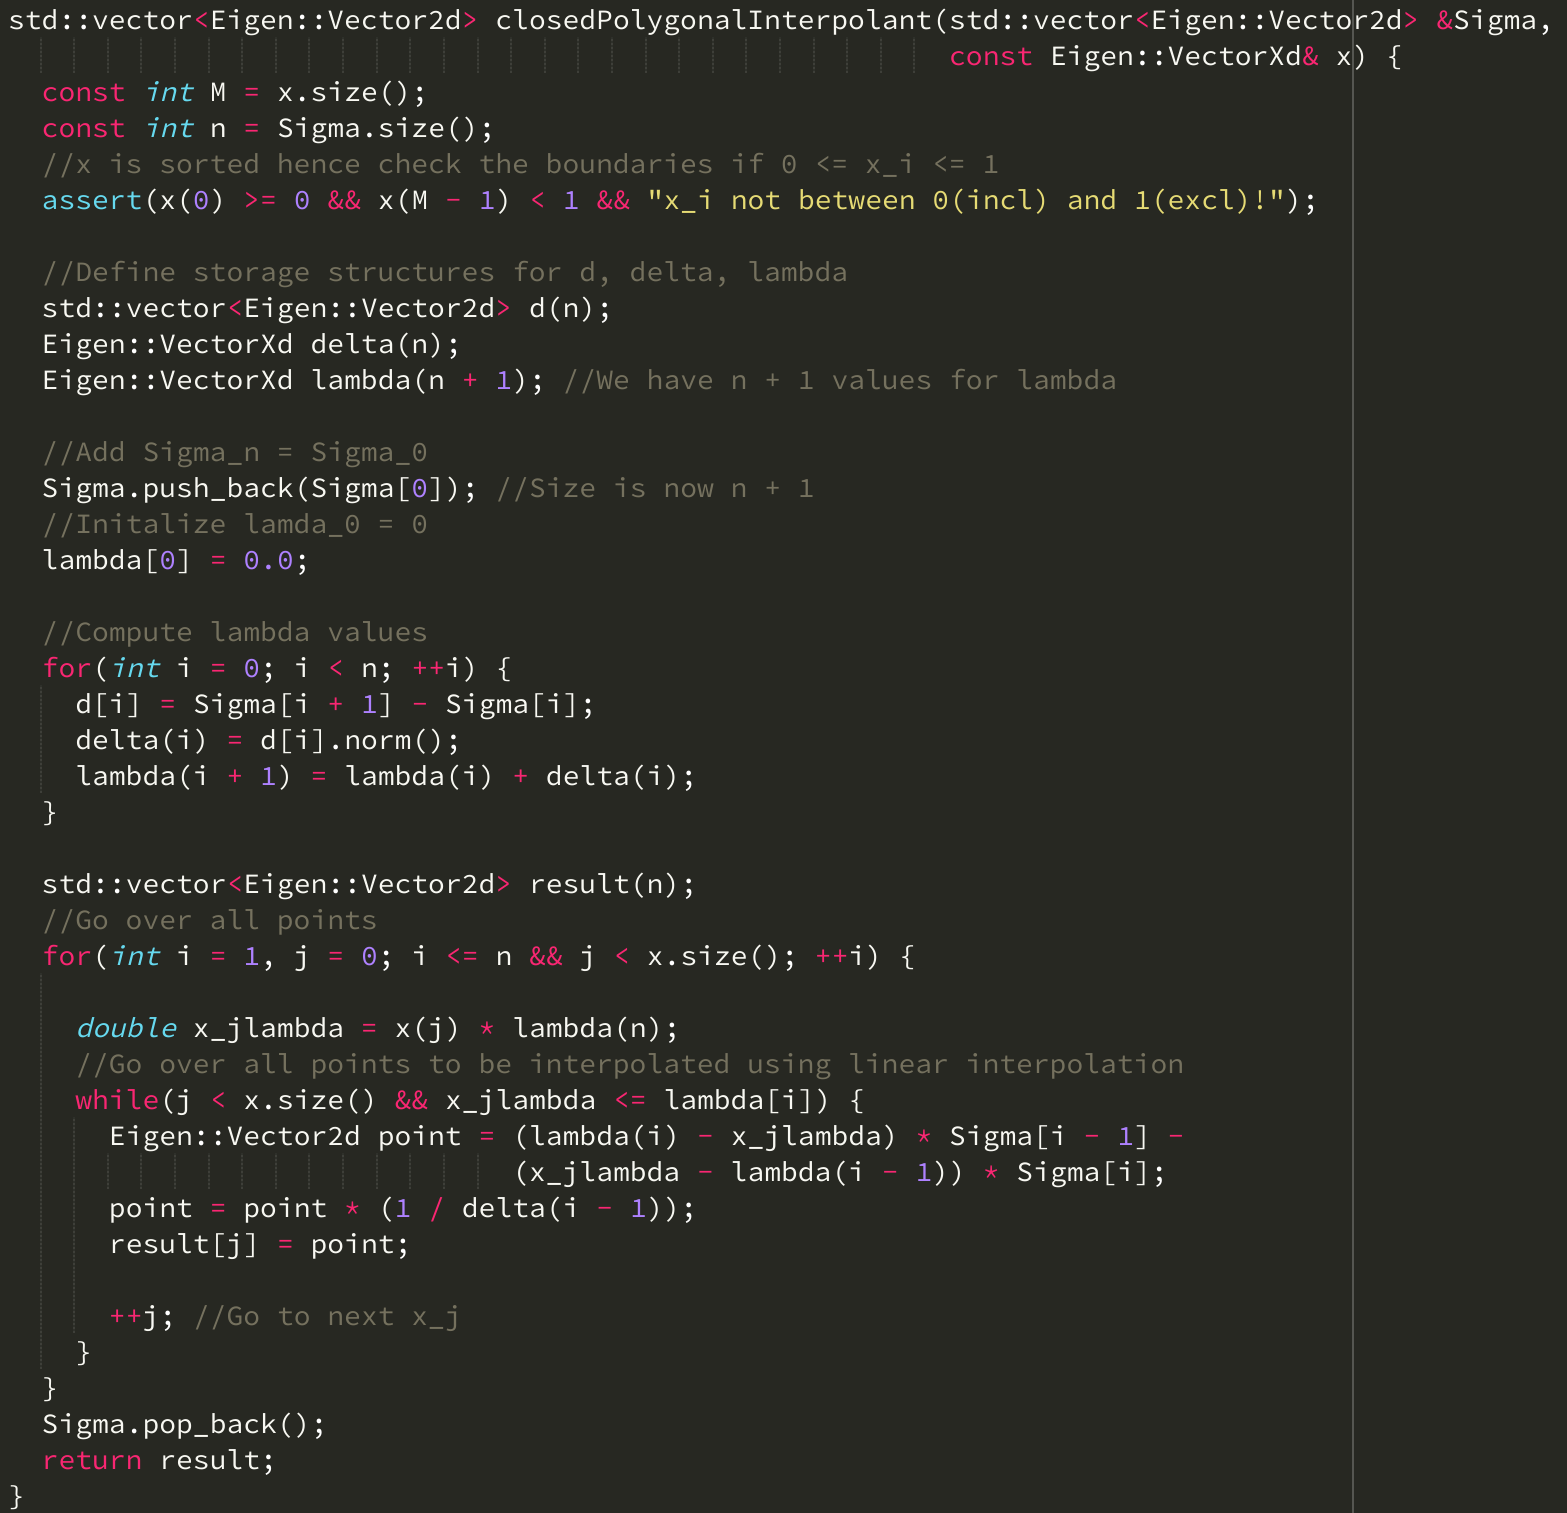
\includegraphics[width=1.0\linewidth]{5-10.a.png}
\end{figure}

\pagebreak

\subsection*{5-10.b}
In this tasked we are tasked to do the same as in the previous task but using a cubic Hermite polynomial interpolant instead of a linear interpolant. We are given a function \verb|hermloceval| which takes arguments \verb|t|, \verb|t1|, \verb|t2|, \verb|y1|, \verb|y2|, \verb|c1| and \verb|c2| and allows us to evaluate the following equation for the local representation of piecewise cubic Hermite interpolant (5.3.3.4)
\begin{equation*}
    s\left(t\right) = y_{i-1}H_{1}\left(t\right) + y_{i}H_{2}\left(t\right) + c_{i-1}H_{3}\left(t\right) + c_{i}H_{4}\left(t\right)
\end{equation*}
hence we can reuse the code of exercise 5-10.a and only have to determine the arguments to the function \verb|hermloceval|. The points $y_{i-1}$ and $y_{i}$ are the same as before and correspond to $\mathbf{p}_{i-1}$ and $\mathbf{p}_{i}$. The slopes $c_{i-1}$ and $c_{i}$ must be computed as defined in section 5.3.3.7 as
\begin{equation*}
    c_{i} = 
    \begin{cases}
    \Delta_{1} &,\text{ for } i = 0 \\
    \Delta_{n} &,\text{ for } i = n \\
    \frac{t_{i+1} - t_{i}}{t_{i+1}-t_{i-1}}\Delta_{i} + \frac{t_{i} - t_{i-1}}{t_{i+1}-t_{i-1}}\Delta_{i+1} \quad &,\text{ if } 1 \leq i \leq n
    \end{cases} \quad , \Delta_{j} := \frac{y_{j} - y_{j - 1}}{t_{j} - t_{j-1}}\,,\: j = 1, \dots, n
\end{equation*}
We know do two things we want to interpolate values $x_{i}$ somewhere onto the polygon, hence we must both interpolate for the $x$-coordinate and the $y$-coordinate. We hence must compute two slopes, one relative to the $x$-coordinate and one relative to the $y$-coordinate. We get the slope for the $x$-coordinate as (for $1 \leq i \leq n$)
\begin{align*}
c_{i} &=
   \frac{t_{i+1} - t_{i}}{t_{i+1}-t_{i-1}}\frac{y_{i} - y_{i - 1}}{t_{i} - t_{i-1}} + \frac{t_{i} - t_{i-1}}{t_{i+1}-t_{i-1}}\frac{y_{i+1} - y_{i}}{t_{i+1} - t_{i}} \\
   &= \frac{1}{t_{i+1} - t_{i - 1}}\left(\frac{\left(t_{i+1} - t_{i}\right) \left(y_{i}-y_{i-1}\right)}{t_{i}-t_{i-1}} + \frac{\left(t_{i}-t_{i-1}\right)\left(y_{i+1} - y_{i}\right)}{t_{i+1} - t_{i}}\right)  \\
   &=  \frac{1}{\delta_{i} + \delta_{i-1}}\left(\frac{\delta_{i} \cdot \mathbf{d}_{i-1} }{\delta_{i-1}} + \frac{\delta_{i-1}\cdot\mathbf{d}_{i}}{\delta_{i}}\right)
\end{align*}

\noindent After having computed the slopes  we can then use \verb|hermloceval| to get both the $x$-coordinate and the $y$-coordinate of the interpolated point. We use $\Sigma_{i, x}$ and $\Sigma_{i, y}$ respectively for this. Most of the code stays the same though, the slopes are computed as follows. 

\begin{figure}[!hbt]
    \centering
\includegraphics[width=1.0\linewidth]{5-10Slopes.png}
\end{figure}

\pagebreak

\noindent We then compute the interpolated points using the same for / while loop structure as before, but computing the points differently, which produces the following code.

\begin{figure}[!hbt]
    \centering
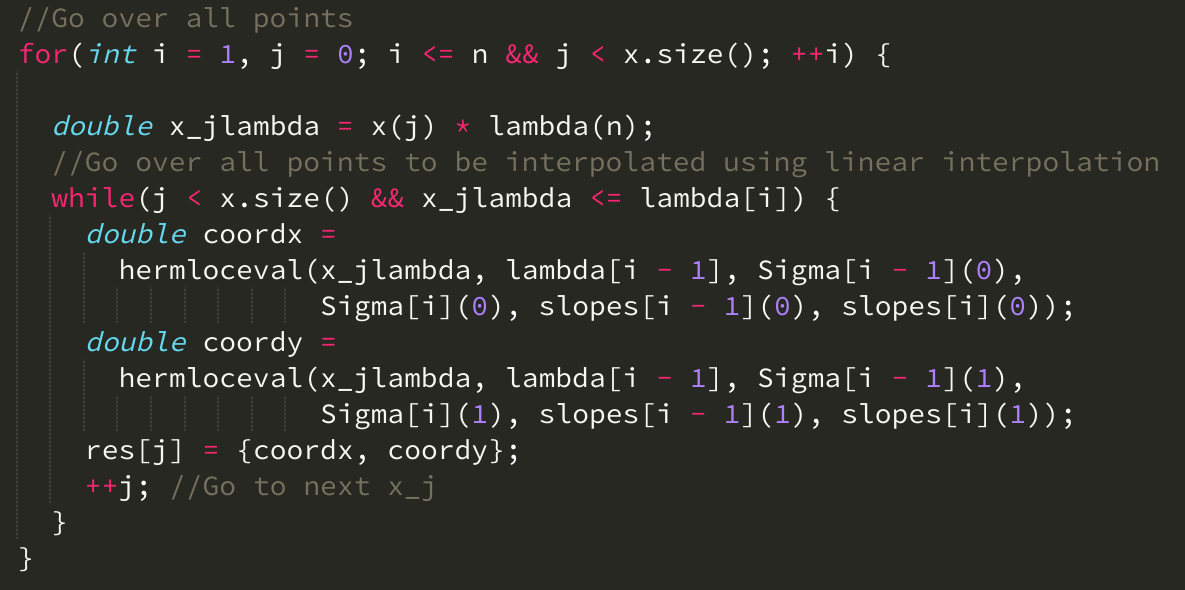
\includegraphics[width=1.0\linewidth]{5-10.b.png}
\end{figure}

\subsection*{5-10.c}
We are given the following piece of pseudocode.

\begin{figure}[!hbt]
    \centering
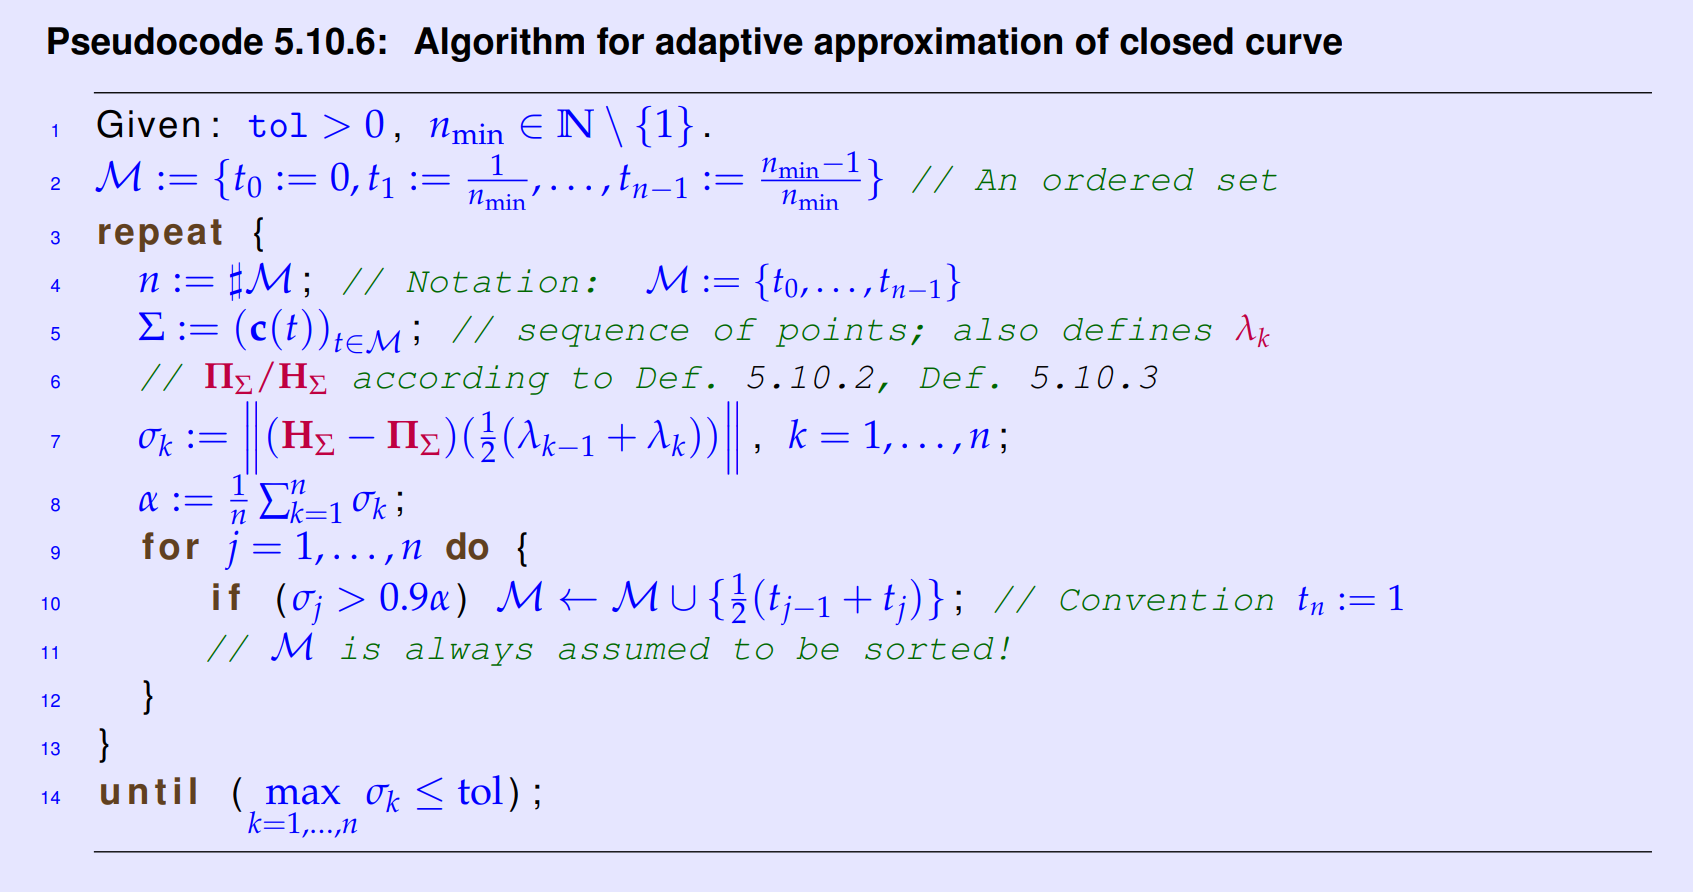
\includegraphics[width=1.0\linewidth]{AlgorithmApproxClosedCurve.png}
\end{figure}

\noindent We are tasked to implement a function \verb|adaptedHermiteInterpolant| based on the two above implementations, which performs the interpolation of a closed curve using the above algorithm in pseudocode. We first see that the set $\mathcal{M}$ is given by 
\begin{equation*}
    \mathcal{M} = \left\{0, \frac{1}{n_{\text{min}}}, \frac{2}{n_{\text{min}}}, \dots, \frac{n_{\text{min}} - 1}{n_{\text{min}}}\right\}
\end{equation*}

\noindent This is \verb|Eigen::VectorXd::LinSpaced(nmin + 1, 0, 1)| in Eigen. We then realize the do / while loop using a vector \verb|dev| to store all $\sigma_{k}$ and the loop condition \verb|dev.maxCoeff() > tol|. We can then use the given functor \verb|c| to evaluate the curve at the linearly spaced points contained in $\mathcal{M}$.

\begin{figure}[!hbt]
    \centering
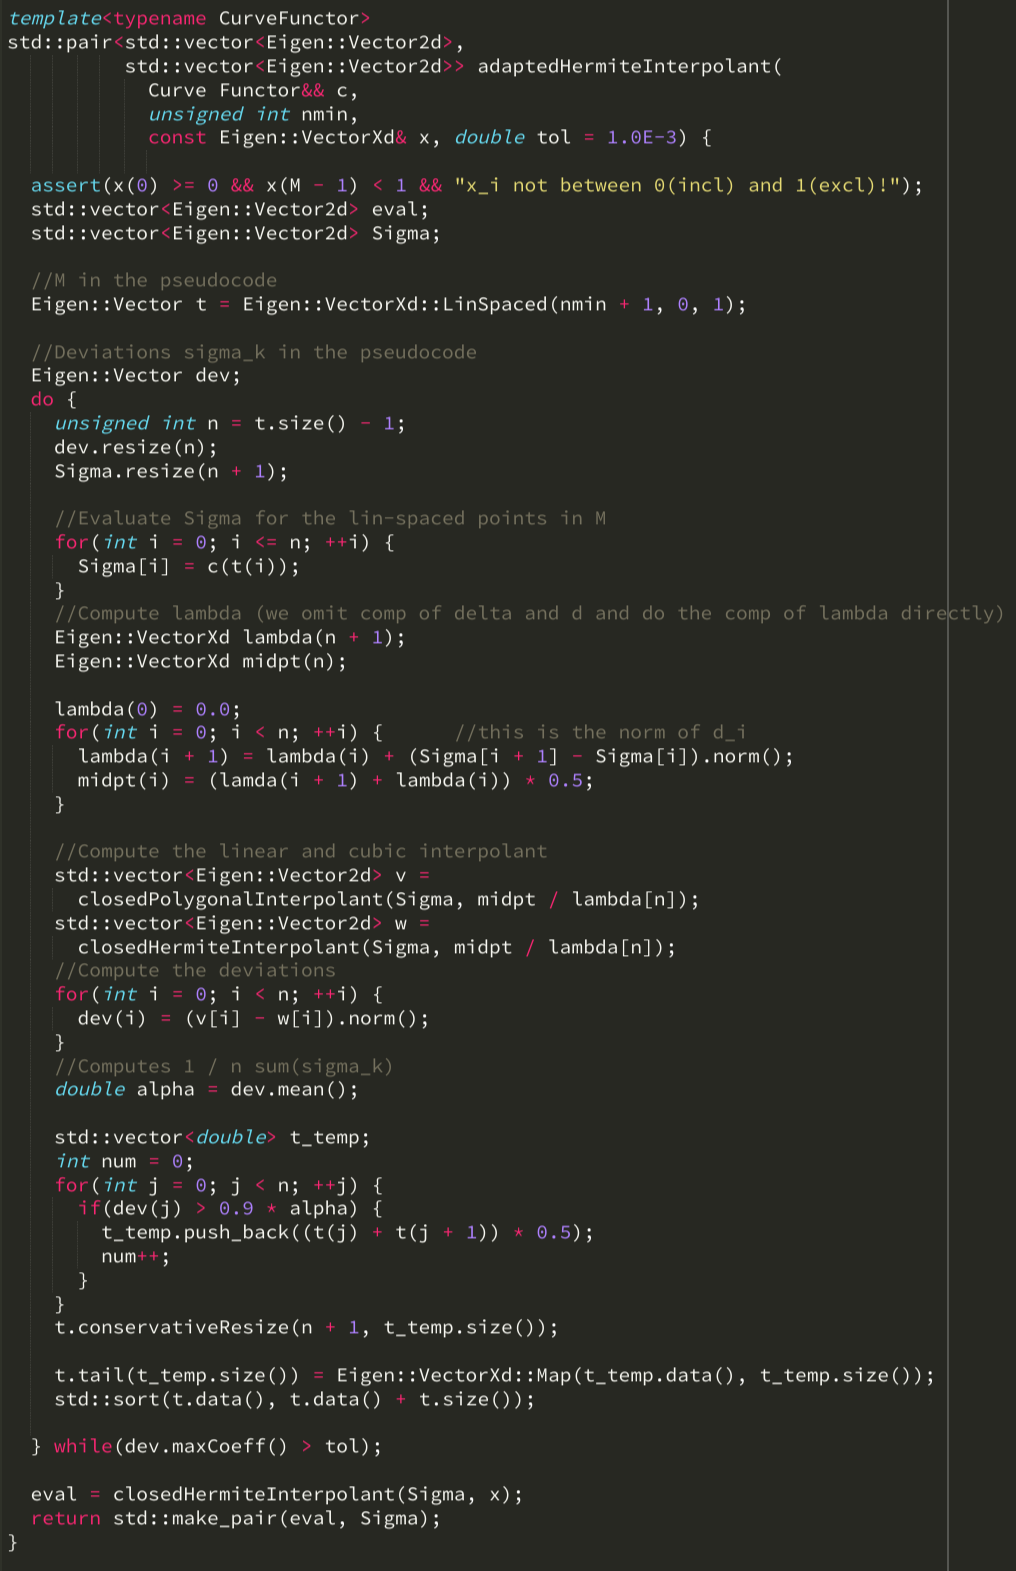
\includegraphics[width=0.9\linewidth]{5-10.c.png}
\end{figure}
\end{document}
